\chapter{Future Work}

\section{Sensors and MCUs}

A proposed alternative to the Arduino MKR1010 is an upgrade to an ESP32 device. An ESP32-WROOM-32 upgrade offers serious improvements over the Arduino MKR1010 in applications needing efficient processing, reduced latency, and energy savings. ESP32 outperforms MKR1010 with a dual-core 240 MHz processor, as opposed to MKR1010's single-core 48 MHz, and a larger RAM capacity of 520 KB against 32 KB. The increased computational power of the ESP32 enables it to do some real-time computations, like running Kalman filters, onboard without the use of an external computer. This removes the high latency and network dependency associated with the MKR1010-based method, where sensor data has to travel to a laptop for processing.
\par
The ESP32 also boasts significantly improved connectivity capabilities that include Wi-Fi and Bluetooth v4.2/BLE. With its dual-mode Wi-Fi operation (STA + AP), the ESP32 allows asynchronous network scanning without interrupting the active connections, which the MKR1010 cannot do. This allows for continuous data transmission while keeping the power consumption low by using intermittent Wi-Fi.
\par
Also, it reduces the system complexity since the ESP32 eliminates the use of external PCs, making deployment and integration easier. The performance and scalability increase because of its capability to handle real-time updates on its own. At a lower cost of ~\$5-10 with more I/O pins, 36 compared to 22, the ESP32 presents an economical, high-performance solution.
\par
Among several conclusions, it is considered that the migration to the ESP32-WROOM-32 avoids limitations concerning latency, energy usage, and system complexity brought into perspective by MKR1010, adding computational efficiency that makes this board definitely superior for real-time application employment. \cite{brownlee_2023_numpy}

\section{Synthetic Data Generation}
In order to improve the quality of our synthetic data so it better mimics real life data, there are several things that can be improved.
Firstly, the velocity equation used, and trajectory could be improved to be more complex and to be better mimic real-life velocity and trajectory of a person going up a spiral. However, since these are modeled by mathematical equations, they cannot model the random behavior of human behavior. 
\par
Another adjustment would be to better model the noise added by the different sensors. In the datasheet, the average and the standard deviation of said noise is mentioned because it can be modeled as additive white gaussian noise, however in real life noise generated by the sensor might be more complex. To add noise to our synthetic data that can more accurately copy real-life noise created by the sensors, deep learning can be used. 
\par
Generative AI can help create realistic sensor noise. By training on a dataset collected from still sensors - where acceleration is zero and pressure, gravity, and the magnetic field are constant - Generative AI could replicate the noise profile. To account for variability due to factors like temperature or sensor orientation, data collection should be repeated on different days and in different positions. 
\cite{tang_2024_synthetic} describes creating a synthetic IMU dataset simulating a person falling. The dataset was trained using SLAM data recorded in an environment free from occlusions. Similarly, we could collect SLAM and IMU data to isolate sensor noise and use it to train a model capable of generating highly realistic IMU noise. In \cref{LSTM_synthdata} the structure of the LSTM model used to generate synthetic data can be seen and \cref{setup_synthdata} shows the experimental set up used.
\begin{figure}[h] 
	\centering 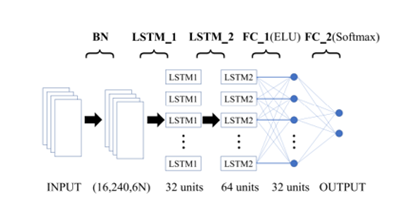
\includegraphics[height=4cm]{./images/LSTMsynth.png}
	\caption{The LSTM architecture used for generating the synthetic data.}
	\label{LSTM_synthdata}
\end{figure}
\begin{figure}[h] 
	\centering 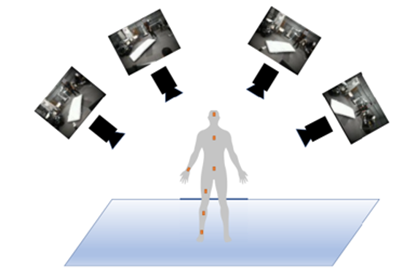
\includegraphics[height=4cm]{./images/setupsynth.png}
	\caption{The experimental setup used for generating the synthetic data.}
	\label{setup_synthdata}
\end{figure}

\section{Data Collection and Processing}
For the future there are several points to improve upon both for data collection and pre-processing. 
For Data collection:

\begin{itemize}
  \item Data collection could be done using more accurate SLAM tools instead of an iPhone. An example of such a tool would be a high-quality stereo camera with LIDAR. This would help improve the accuracy of the data measured.
  \item Generate synthetic variations of the collected dataset to simulate different scenarios. So, using data augmentation, we would create different datasets from an originally measured one to increase and vary our dataset.
\end{itemize}

For pre-processing:

\begin{itemize}
  \item As mentioned before, the method used for synchronization of the ground truth and the raw data was not perfect as it was coarse tuning. Therefore, a fine-tuning method can be applied. This first starts by resampling one of the two signals so that they both have the same sampling frequency. This is crucial because the next step is performing the cross correlation of the signals, and to do that, the signals should have a constant and equal sampling frequency. Performing the cross correlation informs us of how much the 2 signals lag each other, and we can then shift one of the signals by that time to match them. This will help synchronize the signals properly. \cite{yan_2019_ronin}
\end{itemize}

\section{Position Estimation}
The implemented positioning system can be improved via various methods, however, given the scope and requirements of the project, we propose a few main future improvements to the system. 

Firstly, a major issue facing the positioning system, is the inaccuracies of the mathematical spiral model. In order to improve this aspect of the system, a machine learning model can be trained in order to predict positions along the spiral more accurately than a constant mathematical model, and can better reflect the inconsistencies and intricacies of the ground truth data.

Secondly, another issue the system faces, is the lack of usefulness of the accelerometer data due to the high noise levels which causes excessive drift. To combat this, a common method explored in the literature is step counting, which employs situational assumptions about human movement in order to more accurately apply dead reckoning based positioning using IMU data. To implement this, an IMU would need to be rigidly attached to the foot of the user ideally, however if this was infeasible, methods attempting step counting using head-attached IMUs can be explored. \cite{huang_2022_improvement, tiwari_2022_a}
Thirdly, the implemented simple Kalman filtering scheme fails to capture non-linear behavior exhibited by the system, and so implementing an Unscented Kalman filter \cite{bernalpolo_2019_kalman} can improve the performance of the system by improving the system's robustness to non-linear effects.

Finally, a trivial improvement which can be implemented to increase the performance of the overall system, is to replace the used sensors with better performing consumer grade sensors. As an example, the BNO085 is a similar IMU to the used BNO055 with better performance, and within the same price range.


\section{Orientation Estimation}
Future work in terms of the orientation estimation mainly should focus on improving the heading axis accuracy. The heading axis faces the largest issues in performance as seen in our evaluations, which is due to the two reasons discussed earlier. Resolving the issues due to the lack of a baseline vector in the form of the gravity vector will mainly involve implementing a more accurate baseline system based on magnetometer data or integrating different sensors that allow for accurate measurements on the heading axis. An example of this could be integration of spatially spaced sensors, and employing time-difference-of-arrival (TDoA) methods to measure the heading angle. \cite{stanculeanu_2012_enhanced} Furthermore, machine learning methods can be employed in order to improve prediction fidelity, and to learn non-trivial patterns from the dataset. \cite{yan_2019_ronin}

